\documentclass{article}

\usepackage{graphicx}
\usepackage{tikz}
\usepackage{tikzsymbols}
\usetikzlibrary{calc,patterns,shapes.geometric}
\pagestyle{empty}
\usepackage[margin=0pt]{geometry}
\geometry{papersize={14in,12in}}

\def\centerarc[#1](#2)(#3:#4:#5){\draw[#1] ($(#2)+({#5*cos(#3)},{#5*sin(#3)})$) arc (#3:#4:#5);}

\begin{document}
	\begin{figure}
		\centering
		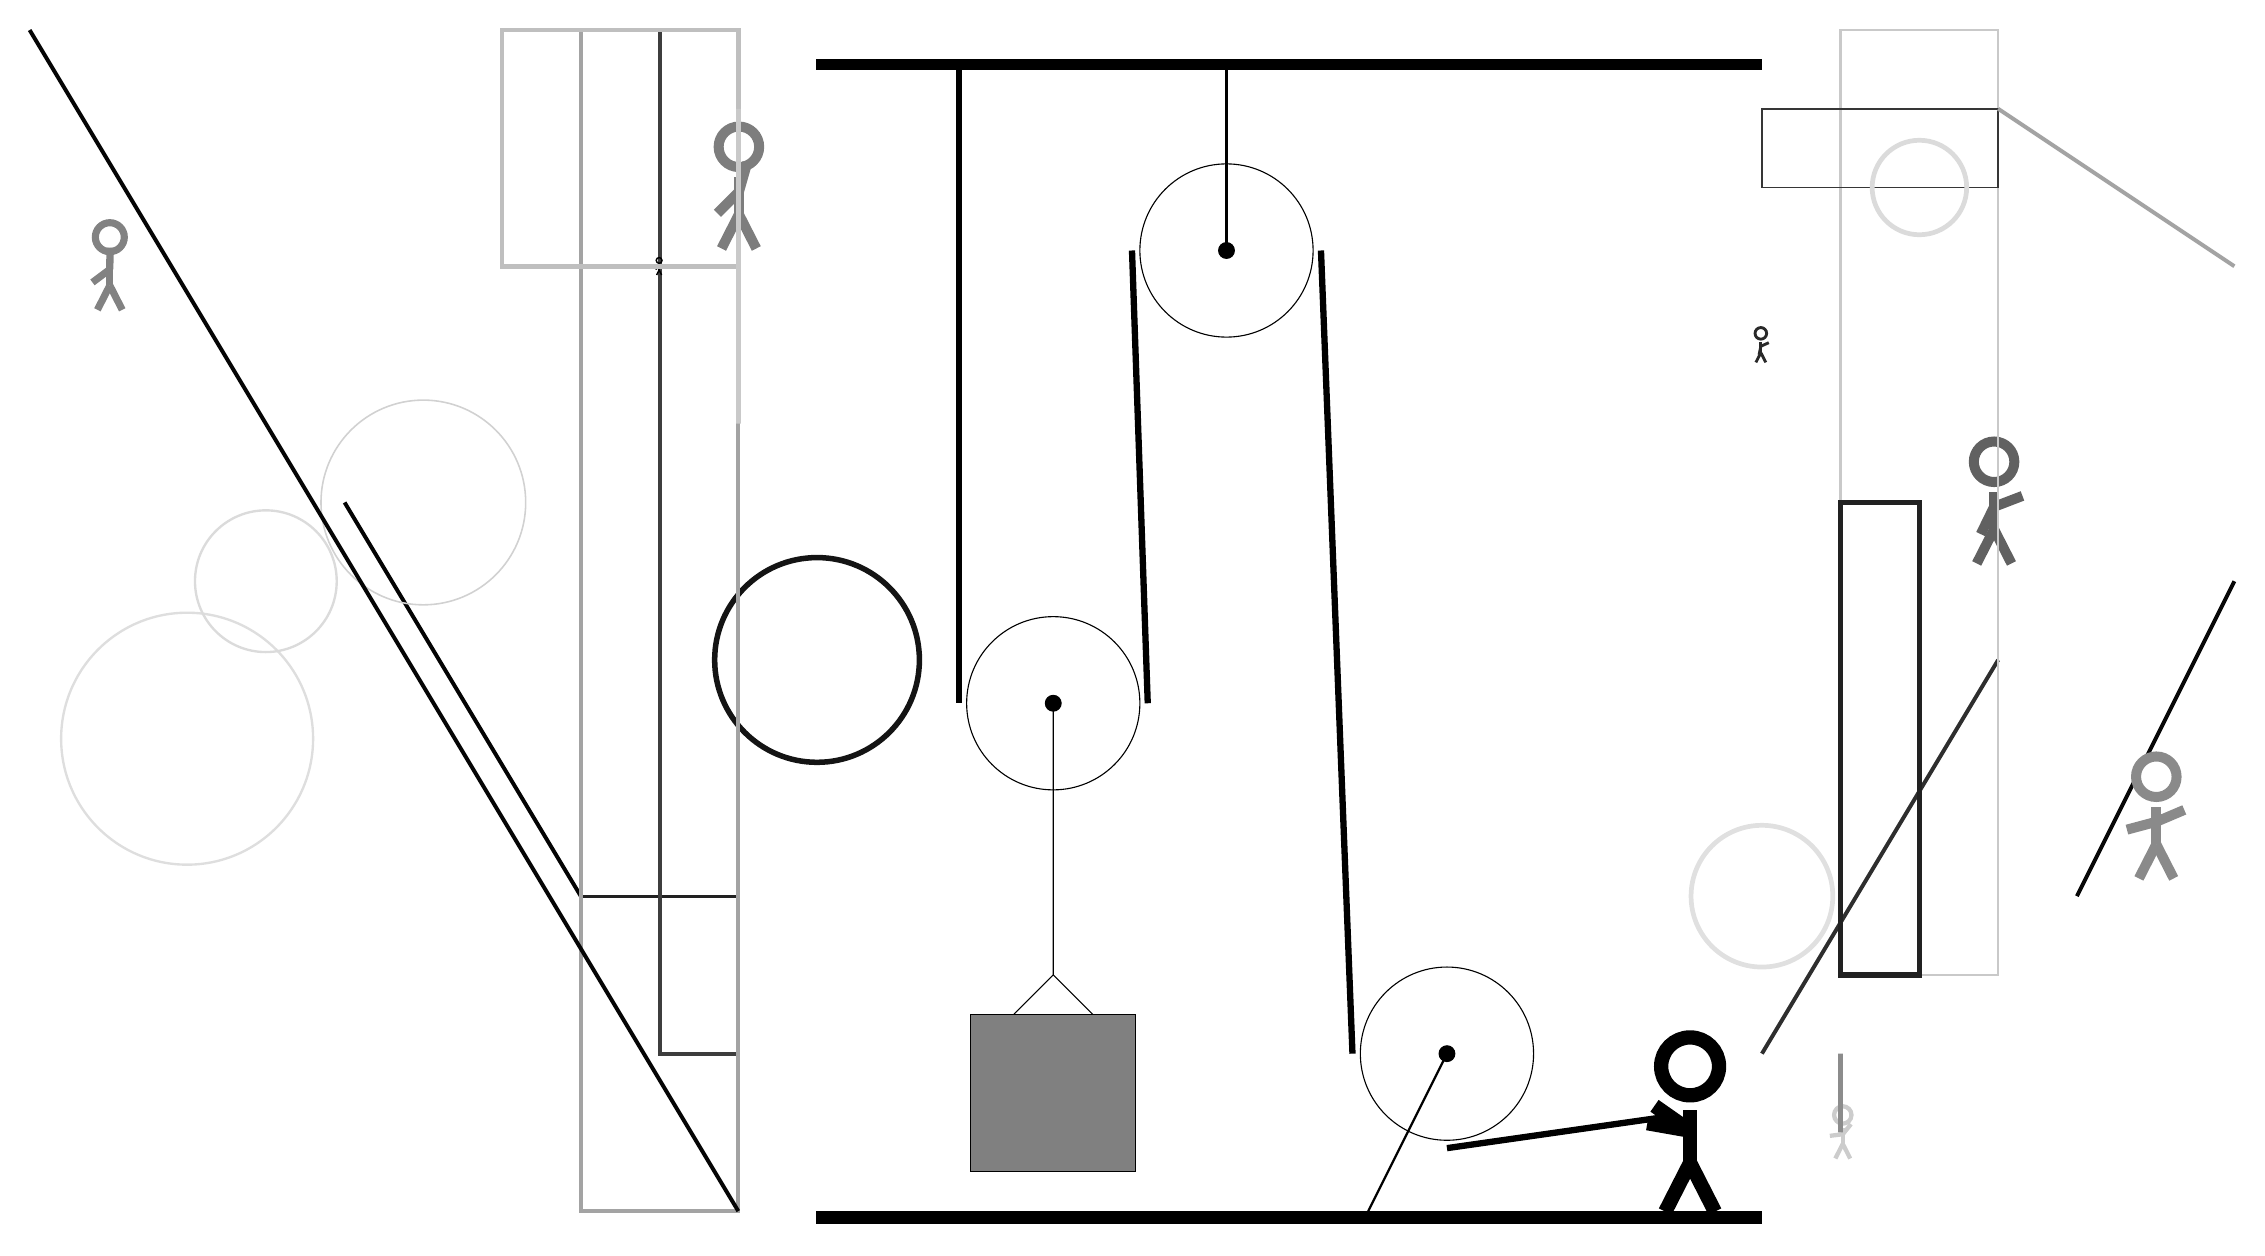
\begin{tikzpicture}
			%%%%% START %%%%%
			
			\draw[fill=black] (-2, 11.5) rectangle (10, 11.625);
			
			\draw (3.2, 9.2) circle (1.1);
			\draw[fill=black] (3.2, 9.2) circle (0.1);
			\draw[thick] (3.2, 9.2) -- (3.2, 11.5);
			
			\draw (6, -1) circle (1.1);
			\draw[fill=black] (6, -1) circle (0.1);
			\draw[thick] (6, -1) -- (5, -3);
			
			\draw (1, 3.45) circle (1.1);
			\draw[fill=black] (1, 3.45) circle (0.1);
			
			\draw[line width=0.5mm, color=black!99](-5, 1) -- (-8, 6);
			
			\draw[line width=0.5mm, color=black!82](13, 4) -- (10, -1);
			\draw [line width=0.3mm, color=black!13](-10, 3) circle (1.6);
			\draw[line width=0.4mm, color=black!87] (-3, 1) rectangle (-5, 1);
			\node[line width=0.2mm, color=black!62] at (13, 6) {\Strichmaxerl[7][64][21]};
			\node[line width=0.4mm, color=black!51] at (-3, 10) {\Strichmaxerl[7][45][74]};
			\draw [line width=0.7mm, color=black!92](-2, 4) circle (1.3);
			\draw [line width=0.3mm, color=black!14](-9, 5) circle (0.9);
			\draw[line width=0.3mm, color=black!21] (11, 0) rectangle (13, 12);
			
			\draw[line width=0.5mm, color=black!97](14, 1) -- (16, 5);
			\draw[line width=0.2mm, color=black!79] (10, 10) rectangle (13, 11);
			
			\draw[line width=0.5mm, color=black!76] (-3, 12) rectangle (-4, -1);
			\node[line width=0.6mm, color=black!100] at (-4, 9) {\Strichmaxerl[1][37][0]};
			\draw[line width=0.5mm, color=black!36] (-3, 12) rectangle (-5, -3);
			\node[line width=0.3mm, color=black!46] at (15, 2) {\Strichmaxerl[7][15][23]};
			\draw [line width=0.2mm, color=black!18](-7, 6) circle (1.3);
			\draw [line width=0.6mm, color=black!14](12, 10) circle (0.6);
			\draw[line width=0.5mm, color=black!36](13, 11) -- (16, 9);
			\draw[line width=0.6mm, color=black!25] (-3, 9) rectangle (-6, 12);
			\node[line width=0.5mm, color=black!84] at (10, 8) {\Strichmaxerl[2][78][24]};
			\node[line width=0.6mm, color=black!49] at (-11, 9) {\Strichmaxerl[5][37][89]};
			\draw[line width=0.7mm, color=black!87] (12, 0) rectangle (11, 6);
			\node[line width=0.6mm, color=black!20] at (11, -2) {\Strichmaxerl[3][7][51]};
			\draw[line width=0.5mm, color=black!98](-3, -3) -- (-12, 12);
			\draw[line width=0.6mm, color=black!21] (-3, 7) rectangle (-3, 11);
			
			\draw [line width=0.6mm, color=black!12](10, 1) circle (0.9);
			\draw[line width=0.6mm, color=black!45] (11, -1) rectangle (11, -2);
			
			\draw (1, 3.45) -- (1, 0.0) -- (0.5, -0.5);
			\draw (1, 0.0) -- (1.5, -0.5);
			\draw[fill=black!50] (-0.05, -0.5) rectangle (2.05, -2.5);
			
			\draw[line width=0.8mm] (-0.2, 11.5) -- (-0.2, 3.45);
			\centerarc[line width=0.8mm](1, 3.45)(180:360:1.2000000000000002);
			\draw[line width=0.8mm](2.2, 3.45) -- (2.0, 9.2);
			\centerarc[line width=0.8mm](3.2, 9.2)(0:180:1.2000000000000002);
			\draw[line width=0.8mm](4.4, 9.2) -- (4.8, -1);
			\centerarc[line width=0.8mm](6, -1)(180:270:1.2000000000000002);
			\draw[line width=0.8mm](6, -2.2) -- (8.8, -1.8);
			
			\node at (9, -1.9) {\Strichmaxerl[10][-35][170]};
			
			\draw[fill=black] (-2, -3) rectangle (10, -3.15);
			
			%%%%% END %%%%%
		\end{tikzpicture}
	\end{figure}	
\end{document}